%======================================================================
% CAPITULO 8: ALQUIMIA INVISIBLE - PROTOCOLO DE TRAZABILIDAD SDC-AI
%======================================================================

\chapter{Alquimia Invisible: Protocolo de Trazabilidad y Seguridad}
\label{ch:alquimia}

\notacientifica{La Alquimia Invisible representa la convergión entre la criptografía moderna y las técnicas ancestrales de la esteganografía, creando un sistema de trazabilidad imperceptible pero verificable.}

\section{Resumen Ejecutivo}
\label{sec:ai-resumen}

El protocolo \textbf{Alquimia Invisible (SDC-AI)} es una estrategia de seguridad que implementa una capa de esteganografía digital de alta fidelidad en el ecosistema \sdc{}. Este sistema utiliza técnicas avanzadas de inyección de metadatos y caracteres de ancho cero para crear sellos de trazabilidad que son completamente imperceptibles para el usuario común pero totalmente verificables por el núcleo de seguridad de Sandra Desktop Container.

La Alquimia Invisible responde a una necesidad crítica en entornos empresariales: la capacidad de rastrear el origen y la cadena de custodia de documentos y archivos sin comprometer la usabilidad ni alertar a posibles atacantes. Mientras que los métodos tradicionales de marcado visible (watermarking) pueden ser removidos o manipulados, los sellos invisibles de Alquimia survive a la mayoría de los procesos de transferencia y transformación de datos.

\subsection{Objetivos del Protocolo}

\begin{caja}{Objetivos de Alquimia Invisible}
\begin{enumerate}
\item \textbf{No Repudiación}: Garantizar que el emisor de un documento no pueda negar su autoría.
\item \textbf{Trazabilidad}: Rastrear el flujo de documentos desde su creación hasta su distribución final.
\item \textbf{Integridad}: Detectar cualquier modificación no autorizada después del sellado.
\item \textbf{Transparencia}: Implementar seguridad sin afectar la experiencia del usuario.
\item \textbf{Interoperabilidad}: Mantener la compatibilidad con sistemas externos que procesen los archivos.
\end{enumerate}
\end{caja}

\notacientifica{El sistema fue diseñado para cumplir con los requisitos más exigentes de auditoría forense digital, incluyendo los estándares establecidos por la ISO 27001 y la normativa de protección de datos vigente.}

\subsection{Caso de Uso Empresarial}

Imagine el siguiente escenario: Un empleado de una institución gubernamental genera un informe confidencial sobre nóminas y lo exporta desde el Visor de Documentos de SDC. Semanas después, ese documento aparece en manos no autorizadas. Gracias al protocolo Alquimia Invisible, el equipo de seguridad puede:

\begin{enumerate}
\item Extraer el sello invisible del documento
\item Verificar la identidad del terminal emisor (dirección MAC)
\item Identificar al usuario que realizó la exportación
\item Rastrear la cadena de custodia del archivo
\item Proporcionar evidencia forense admisible en procedimientos legales
\end{enumerate}

Todo esto ocurre sin que el empleado original haya notado nada diferente en su experiencia de usuario, y sin que ningún mecanismo de seguridad visible haya alertado a potenciales atacantes.

\section{Marco Normativo y Estándares Internacionales}
\label{sec:ai-normas}

El desarrollo del protocolo Alquimia Invisible se rige por un marco normativo robusto que asegura el cumplimiento con estándares internacionales de seguridad de la información y protección de datos.

\subsection{ISO/IEC 27001:2022}

La norma ISO 27001 establece los requisitos para un Sistema de Gestión de Seguridad de la Información (SGSI). El protocolo Alquimia Invisible contribuye directamente al cumplimiento de dos controles específicos:

\begin{caja}{Controles ISO 27001 Applicablees}
\begin{itemize}
\item \textbf{Control A.8.25 (Cifrado)}: La implementación cumple con el requisito de proteger la confidencialidad e integridad de la información mediante técnicas criptográficas y de ocultación (Steganography). El sello注入ado en los archivos utiliza algoritmos de hash derivados que garantizan la integridad del mensaje.

\item \textbf{Control A.8.33 (Eliminación de información)}: El diseño del sistema asegura que los metadatos de trazabilidad no interfieran con la utilidad o el propósito primario del archivo. Los caracteres de ancho cero no afectan la estructura de datos, permitiendo que los archivos mantengan su funcionalidad original.
\end{itemize}
\end{caja}

\notacientifica{La implementación de steganografía como capa adicional de seguridad representa una evolución significativa en la protección de información sensible, complementando los controles criptográficos tradicionales con capacidades de ocultación avanzadas.}

\subsection{ISO/IEC 24760-1:2019}

Esta norma establece los principios para la gestión de identidad y trazabilidad. El protocolo Alquimia Invisible implementa soporte para el principio fundamental de \textbf{No Repudiación}:

\begin{definicion}
\textbf{No Repudiación} es la garantía de que el emisor de un mensaje o documento no puede negar posteriormente que lo envió, y que el receptor no puede negar que lo recibió. En el contexto de archivos digitales, esto significa poder demostrar criptográficamente la identidad del origen y la integridad del contenido.
\end{definicion}

\notacientifica{Al inyectar la firma del nodo (dirección MAC del dispositivo) y del usuario (JWT de sesión) de forma invisible, el sistema garantiza que el origen de un archivo sea rastreable hasta el emisor original, proporcionando evidencia forense sólida.}

La inyección de identidad se realiza mediante la combinación de tres elementos:

\begin{enumerate}
\item \textbf{Device ID}: Identificador único del dispositivo emisor, derivado de la dirección MAC
\item \textbf{User ID}: Identificador del usuario extraído del JWT de sesión activo
\item \textbf{Timestamp}: Marca de tiempo Unix de la generación del archivo
\end{enumerate}

Estos tres elementos se combinan mediante una función hash criptográfica (SHA-256) para generar un hash de identidad único que se inyecta en el archivo.

\subsection{Estándar Unicode}

La implementación técnica de Alquimia Invisible respeta rigurosamente el estándar internacional Unicode, asegurando la interoperabilidad de datos sin corromper el parsing de sistemas externos:

\begin{caja}{Caracteres Unicode Utilizados}
\begin{itemize}
\item \textbf{U+200C} (Zero Width Non-Joiner, ZWNJ): Representa el bit 0 en la codificación
\item \textbf{U+200D} (Zero Width Joiner, ZWJ): Representa el bit 1 en la codificación
\item \textbf{U+FEFF} (Byte Order Mark, BOM): Utilizado como marcador de inicio del sello
\item \textbf{U+200B} (Zero Width Space, ZWSP): Utilizado como marcador de fin del sello
\end{itemize}
\end{caja}

\notacientifica{La selección de estos caracteres específicos se basa en su propiedad de ser invisible en la mayoría de editores de texto, navegadores y procesadores de texto. Ninguno de estos caracteres produce renderizado visual, pasando desapercibidos para el usuario común.}

\subsection{COBIT 2019}

El marco de gobernanza COBIT 2019 proporciona directrices para la gestión de TI empresarial. El protocolo Alquimia Invisible se alinea con varios procesos de este marco:

\begin{caja}{Procesos COBIT Applicablees}
\begin{itemize}
\item \textbf{APO12 (Gestión de Riesgos de Seguridad de la Información)}: El protocolo permite la identificación proactiva de amenazas mediante el rastreo de la distribución de información sensible.

\item \textbf{DSS05 (Gestión de Servicios de Seguridad)}: Proporciona protección contra la divulgación no autorizada de información sensible mediante trazabilidad.

\item \textbf{BAI06 (Gestión de Cambios)}: El sistema de actualizaciones atómicas de SDC trabaja en conjunto con Alquimia Invisible para garantizar la integridad de la cadena de suministro de software.
\end{itemize}
\end{caja}

\section{Estrategias de Inyección por Arquitectura de Archivo}
\label{sec:ai-estrategias}

El protocolo Alquimia Invisible implementa diferentes estrategias de inyección según el tipo de archivo a proteger. Esta sección detalla cada metodología técnica, los algoritmos involucrados y las consideraciones de implementación.

\subsection{Alquimia para Documentos Estructurados (PDF)}
\label{sec:ai-pdf}

Los archivos PDF representan uno de los formatos más utilizados para la documentación empresarial. El protocolo implementa la técnica de \textbf{Metadata Object Injection} para insertar sellos de trazabilidad en la estructura interna del documento.

\notacientifica{El formato PDF organiza su contenido en una estructura de objetos llamada Trailer, que contiene metadatos del documento. Esta estructura es editable sin alterar el contenido visual del documento, haciéndola ideal para la inyección de sellos de seguridad.}

\subsubsection{Arquitectura del Trailer PDF}

Un documento PDF contiene las siguientes secciones estructurales:

\begin{enumerate}
\item \textbf{Header}: Identificador de versión del PDF
\item \textbf{Body}: Objetos que contienen el contenido del documento
\item \textbf{Cross-Reference Table}: Tabla de referencias cruzadas
\item \textbf{Trailer}: Metadatos y punteros de lectura
\end{enumerate}

El diccionario de información del documento (Info Dictionary) contiene campos como Author, Creator, Producer, Title y Subject. SDC aprovecha este diccionario para injectar un campo personalizado.

\subsubsection{Implementación Técnica}

La implementación en Rust utiliza la librería \texttt{lopdf} para la manipulación de documentos:

\begin{lstlisting}[language=rust, caption={Inyección de Metadata en PDF}]
use lopdf::Document;

pub fn inject_sdc_seal(document: &mut Document, seal_data: &[u8]) 
-> Result<(), AlquimiaError> {
    
    // Generar el sello a partir de los datos de identidad
    let seal = generate_seal_hash(seal_data)?;
    
    // Obtener referencia al diccionario deInfo
    let info = document.trailer.get(b"Info")
        .and_then(|r| document.get_object(r).ok())
        .and_then(|obj| obj.as_dict().ok())
        .ok_or(AlquimiaError::PDFStructureError)?;
    
    // Crear clave personalizada SDC-Seal
    let key = Object::Name(b"SDC-Seal".to_vec());
    let value = Object::String(seal.to_vec(), String::from_utf8_lossy(&seal).to_string());
    
    // Inyectar el sello en el diccionario
    info.set(key, value);
    
    Ok(())
}

fn generate_seal_hash(data: &[u8]) -> Result<Vec<u8>, AlquimiaError> {
    use sha2::{Sha256, Digest};
    let mut hasher = Sha256::new();
    hasher.update(data);
    Ok(hasher.finalize().to_vec())
}
\end{lstlisting}

\notacientifica{El sello注入ado se convierte en parte permanente de la estructura del PDF. A diferencia de los metadatos visibles que pueden editarse, este sello sobrevive a la mayoría de transformaciones de documentos.}

\subsubsection{Ubicación del Sello PDF}

\begin{caja}{Ubicación del Sello en PDF}
\begin{itemize}
\item \textbf{Target}: Diccionario Info del Trailer
\item \textbf{Clave}: SDC-Seal
\item \textbf{Valor}: Hash criptográfico de 64 bytes (SHA-256)
\item \textbf{Visibilidad}: Invisible al lector (PDF Viewer)
\item \textbf{Accesibilidad}: Detect mediante inspección de objetos binarios
\end{itemize}
\end{caja}

\subsubsection{Caso de Uso: Auditoría de Documentos Oficiales}

Supongamos que una institución financiera distribuye un informe de auditoría a varios departamentos. Cada documento PDF exportado desde SDC lleva注入ado el sello SDC-Seal que incluye:

\begin{enumerate}
\item Identificador del dispositivo emisor
\item Identificador del usuario que realizó la exportación
\item Timestamp de generación
\item Hash del contenido original
\end{enumerate}

Si posteriormente surge una filtración, el equipo de seguridad puede:

\begin{enumerate}
\item Abrir el PDF con una herramienta de análisis binario
\item Localizar el diccionario Info
\item Extraer el valor de la clave SDC-Seal
\item Verificar el hash contra la base de datos de sellos emitidos
\item Rastrear la distribución original del documento
\end{enumerate}

\subsection{Alquimia Esteganográfica para Texto Plano}
\label{sec:ai-texto}

Los archivos de texto plano (CSV, TXT, LOG, y otros formatos de flujo secuencial) requieren un enfoque diferente debido a su estructura simple. El protocolo implementa la técnica de \textbf{Zero-Width Bit Encoding}.

\notacientifica{Los archivos de texto plano no tienen estructura de metadatos como los PDF. Por lo tanto, la inyección debe realizarse mediante la inserción de caracteres invisibles directamente en el flujo del archivo.}

\subsubsection{Principio de Operación}

La técnica de codificación de bits de ancho cero convierte la información del sello en una secuencia de bits que se mapea a caracteres Unicode invisibles:

\begin{caja}{Mapeo de Bits a Caracteres}
\begin{itemize}
\item \textbf{Bit 1}: U+200D (Zero Width Joiner)
\item \textbf{Bit 0}: U+200C (Zero Width Non-Joiner)
\end{itemize}
\end{caja}

La cadena de bits se encapsula entre marcadores de control:

\begin{caja}{Marcadores de Encapsulamiento}
\begin{itemize}
\item \textbf{Inicio}: U+FEFF (Byte Order Mark / BOM)
\item \textbf{Fin}: U+200B (Zero Width Space)
\end{itemize}
\end{caja}

\subsubsection{Proceso de Codificación}

El proceso de codificación transforma el hash de identidad en una secuencia de caracteres invisibles:

\begin{enumerate}
\item \textbf{Generación del Hash}: Se genera un hash SHA-256 de 256 bits (32 bytes)
\item \textbf{Conversión a Bits}: Cada byte se convierte a 8 bits, totalizando 256 bits
\item \textbf{Mapeo}: Cada bit se mapea al carácter Unicode correspondiente (0 → ZWNJ, 1 → ZWJ)
\item \textbf{Encapsulamiento}: Se añade el BOM al inicio y ZWSP al final
\item \textbf{Inserción}: La cadena resultante se concatena al final del archivo
\end{enumerate}

\notacientifica{El resultado es una firma completamente invisible que no altera la apariencia, estructura o funcionalidad del archivo. Un usuario que abra el archivo en cualquier editor de texto, hoja de cálculo o navegador no verá ninguna diferencia.}

\subsubsection{Ejemplo Práctico de Codificación}

\begin{lstlisting}[language=rust, caption={Codificación Zero-Width}]
use std::fs::{File, OpenOptions};
use std::io::Write;

const ZWJ: char = '\u{200D}';  // Bit 1
const ZWNJ: char = '\u{200C}';  // Bit 0  
const BOM: char = '\u{FEFF}';   // Marcador inicio
const ZWSP: char = '\u{200B}'; // Marcador fin

pub fn encode_invisible_signature(hash: &[u8]) -> String {
    let mut signature = String::new();
    
    // Agregar marcador de inicio
    signature.push(BOM);
    
    // Convertir cada byte a 8 bits
    for byte in hash {
        for i in (0..8).rev() {
            let bit = (byte >> i) & 1;
            signature.push(if bit == 1 { ZWJ } else { ZWNJ });
        }
    }
    
    // Agregar marcador de fin
    signature.push(ZWSP);
    
    signature
}

pub fn inject_signature(file_path: &str, signature: &str) 
-> std::io::Result<()> {
    let mut file = OpenOptions::new()
        .append(true)
        .open(file_path)?;
    
    file.write_all(signature.as_bytes())?;
    Ok(())
}
\end{lstlisting}

\subsubsection{Características de Invisibilidad}

La técnica de Zero-Width Bit Encoding ofrece características de invisibilidad superiores:

\begin{caja}{Propiedades de Invisibilidad}
\begin{itemize}
\item \textbf{No altera la estructura}: No añade líneas adicionales ni modifica el formato
\item \textbf{No visible en editores}: Todos los editores de texto interpretan estos caracteres como no reproducibles
\item \textbf{No altera hojas de cálculo}: Las celdas mantienen su contenido y formato
\item \textbf{Sobrevive copy-paste}: Los caracteres se copian junto con el texto
\item \textbf{Resiste procesos de transferencia}: FTP, HTTP, email no alteran los caracteres Unicode
\end{itemize}
\end{caja}

\notacientifica{Esta técnica ha sido probada extensivamente con múltiples transferencias: upload/download via FTP, envío por email (SMTP/POP3/IMAP), compartición via Dropbox/Google Drive, y edición en Microsoft Excel, Google Sheets, y LibreOffice Calc. En todos los casos, la firma sobrevivió intacta.}

\subsubsection{Ejemplo Visual}

Considere un archivo CSV simple:

\begin{verbatim}
nombre,apellido,monto
Juan,Perez,5000
Maria,Gomez,7500
\end{verbatim}

Después de la inyección de Alquimia Invisible, el archivo se ve idéntico:

\begin{verbatim}
nombre,apellido,monto
Juan,Perez,5000
Maria,Gomez,7500
\end{verbatim}

Pero en términos de bytes, contiene (representación visual):

\begin{verbatim}
nombre,apellido,monto
Juan,Perez,5000
Maria,Gomez,7500[ZWSP][ZWJ][ZWNJ]...[BOM]
\end{verbatim}

El usuario no ve nada diferente, pero el sistema puede extraer la firma de trazabilidad.

\section{Especificaciones de Seguridad de la Capa}
\label{sec:ai-especificaciones}

Esta sección detalla las propiedades cryptográficas y de seguridad del protocolo Alquimia Invisible.

\subsection{Integridad mediante Hashing}

El sello injectado incluye un hash derivado de la identidad del usuario y del terminal. Cualquier intento de modificar el sello sin las llaves del contenedor invalidará la secuencia de bits detectada por el validador en Rust.

\notacientifica{La invalidez del sello puede detectarse en milisegundos, permitiendo la identificación inmediata de archivos comprometidos.}

\begin{caja}{Proceso de Verificación de Integridad}
\begin{enumerate}
\item \textbf{Extracción}: Se extraen los caracteres invisibles del archivo
\item \textbf{Decodificación}: La secuencia se convierte de nuevo a bits
\item \textbf{Extracción de datos}: Se separan el hash original del contenido
\item \textbf{Recálculo}: Se calcula el hash esperado con las credenciales actuales
\item \textbf{Comparación}: Se comparan ambos hashes
\item \textbf{Resultado}: Válido (coinciden) o Inválido (no coinciden)
\end{enumerate}
\end{caja}

\subsection{Resistencia a la Detección}

El protocolo ha sido diseñado para resistir intentos de detección:

\begin{caja}{Características Anti-Detección}
\begin{itemize}
\item \textbf{Sin caracteres ASCII extendidos}: Evita generar alertas en sistemas de detección de malware
\item \textbf{Sin saltos de línea adicionales}: Sobrevive a procesos que normalizan archivos
\item \textbf{Uso exclusivo de UTF-8}: Compatible con cualquier sistema que soporte Unicode
\item \textbf{Densidad variable}: La longitud del sello puede ajustarse según necesidades
\end{itemize}
\end{caja}

\notacientifica{Los sistemas tradicionales de Prevención de Pérdida de Datos (DLP) buscan patrones como palabras clave sensibles o secuencias hexadecimales específicas. Los caracteres de ancho cero no activan estas alertas porque son técnicamente "vacíos" desde la perspectiva del renderizado.}

\subsection{No Repudiación Global}

Cada archivo generado por SDC lleva implícita la "huella digital" del terminal origen:

\begin{caja}{Elementos de No Repudiación}
\begin{itemize}
\item \textbf{MAC Address}: Identificador único de la tarjeta de red del dispositivo
\item \textbf{JWT de Sesión}: Token de autenticación del usuario
\item \textbf{Timestamp}: Fecha y hora exacta de generación
\item \textbf{Versión de SDC}: Versión del contenedor utilizada
\item \textbf{Hash de Contenido}: Hash SHA-256 del contenido original
\end{itemize}
\end{caja}

\notacientifica{Esta combinación de elementos hace prácticamente imposible que un usuario niegue la autoría o exportación de un documento, ya que toda la información necesaria para verificar la identidad está contenida en el propio archivo.}

\subsection{Fallback de Descifrado Dual-Key}

Para garantizar la interoperabilidad con paquetes antiguos o generados en dispositivos externos, el motor de ingesta implementa un sistema de fallback:

\begin{caja}{Estrategia Dual-Key}
\begin{enumerate}
\item \textbf{Intento primario}: Descifrar usando Device Secret actual
\item \textbf{Intento secundario}: Si falla, usar MAC Address como clave de respaldo
\item \textbf{Resultado}: Si cualquiera de los dos succeed, el archivo se procesa normalmente
\end{enumerate}
\end{caja}

\notacientifica{Este mecanismo asegura que archivos generados en dispositivos anteriores a una actualización de seguridad puedan仍然 ser procesados, mientras mantiene la seguridad para nuevos archivos.}

\section{Guía de Auditoría Forense Digital}
\label{sec:ai-auditoria}

Esta sección proporciona instrucciones detalladas para auditores que necesitan validar la firma de Alquimia Invisible sin acceso a las herramientas de Sandra Desktop Container.

\notacientifica{Los métodos descritos a continuación permiten la verificación manual de sellos, proporcionando evidencia admisible en procedimientos forenses y legales.}

\subsection{Método de Extracción Hexadecimal}

La forma más directa de verificar la presencia del sello es mediante inspección hexadecimal:

\begin{enumerate}
\item \textbf{Localizar el marcador de inicio}: Buscar la secuencia \texttt{EF BB BF} (representación hexadecimal del BOM U+FEFF)
\item \textbf{Identificar el patrón de datos}: Secuencias repetitivas de:
   \begin{itemize}
   \item \texttt{E2 80 8C} = ZWNJ (bit 0)
   \item \texttt{E2 80 8D} = ZWJ (bit 1)
   \end{itemize}
\item \textbf{Localizar el marcador de fin}: Buscar \texttt{E2 80 8B} (ZWSP)
\end{enumerate}

\notacientifica{Estos patrones hexadecimales son consistentes y universales, permitiendo la detección en cualquier archivo que haya sido procesado por el protocolo Alquimia Invisible.}

\subsection{Comando Bash de Auditoría}

Para auditorías automatizadas, se recomienda el siguiente comando:

\begin{lstlisting}[language=bash, caption={Comando de Auditoría}]
#!/bin/bash
# Archivo: audit_alquimia.sh
# Uso: ./audit_alquimia.sh <archivo>

FILE=$1
BYTES=1000

echo "=== Auditoría Alquimia Invisible ==="
echo "Archivo: $FILE"
echo ""

# Extraer los últimos bytes y buscar preámbulo BOM
echo "Buscando marcador de inicio (BOM)..."
tail -c $BYTES "$FILE" | xxd -p | grep "efbbbf" && \
echo "[+] Marcador BOM encontrado" || \
echo "[-] Marcador BOM no encontrado"

# Verificar presencia de secuencias ZWJ/ZWNJ
echo ""
echo "Buscando secuencia de bits..."
tail -c $BYTES "$FILE" | xxd -p | grep -E "(e2808c|e2808d)" && \
echo "[+] Secuencia de bits detectada" || \
echo "[-] Secuencia de bits no encontrada"

# Mostrar los últimos bytes del archivo
echo ""
echo "Últimos 100 bytes (hex):"
tail -c 100 "$FILE" | xxd | tail -5
\end{lstlisting}

\notacientifica{Este script puede integrarse en pipelines de CI/CD para verificar automáticamente la presencia de sellos de trazabilidad en archivos críticos.}

\subsection{Validación Manual Paso a Paso}

Para una validación manual sin herramientas especializadas:

\begin{enumerate}
\item \textbf{Abrir el archivo en un editor hexadecimal}: Como HxD, Hex Fiend, o CyberChef
\item \textbf{Navegar al final del archivo}: Donde se ubica la firma invisible
\item \textbf{Buscar caracteres UTF-8 específicos}:
   \begin{itemize}
   \item Buscar \texttt{EF BB BF} (BOM = inicio de firma)
   \item Identificar patrones de \texttt{80 8C} y \texttt{80 8D}
   \item Localizar \texttt{80 8B} (fin de firma)
   \end{itemize}
\item \textbf{Extraer la secuencia}: Copiar los bytes entre BOM y ZWSP
\item \textbf{Convertir a caracteres}: Interpretar la secuencia como bits
\item \textbf{Verificar contra base de datos}: Comparar con registros conocidos
\end{enumerate}

\notacientifica{La validación manual es especialmente útil en situaciones donde se requiere evidencia para procedimientos legales, ya que puede repetirse independientemente.}

\subsection{Casos de Prueba para Validación}

Para verificar la implementación correcta del protocolo, se recomienda ejecutar los siguientes casos de prueba:

\begin{caja}{Casos de Prueba}
\begin{enumerate}
\item \textbf{CT-01}: Generar archivo CSV nuevo → Verificar presencia de sello → OK
\item \textbf{CT-02}: Exportar PDF desde Visor → Verificar clave SDC-Seal → OK
\item \textbf{CT-03}: Modificar archivo sellado → Verificar invalidez → OK
\item \textbf{CT-04}: Transferir archivo por FTP → Verificar supervivencia → OK
\item \textbf{CT-05}: Abrir en Excel/Sheets → Guardar → Verificar sello intacto → OK
\item \textbf{CT-06}: Enviar por email → Recibir → Verificar sello → OK
\item \textbf{CT-07}: Copy-paste contenido → Verificar sello en copia → OK
\end{enumerate}
\end{caja}

\notacientifica{Estos casos de prueba cubren los escenarios más comunes de manipulación y transferencia de archivos. La implementación debe pasar todos los casos para considerarse lista para producción.}

\section{Casos de Uso y Ejemplos Reales}
\label{sec:ai-casos}

Esta sección presenta casos de uso empresarial concretos que demuestran el valor del protocolo Alquimia Invisible.

\subsection{Caso de Uso 1: Seguimiento de Documentos Officiales}

\textbf{Escenario}: Una institución gubernamental emite informes mensuales de gestión a diferentes dependencias.

\begin{caja}{Flujo de Trabajo}
\begin{enumerate}
\item Funcionario genera informe en SDC Visor
\item Sistema injecta sello con ID de usuario, dispositivo y timestamp
\item Documento se distribuye por correo electrónico seguro
\item Semanas después, el documento aparece en medios no autorizados
\item Equipo de seguridad extrae el sello del documento
\item Se identifica al usuario y dispositivo de origen
\item Se inicia investigación interna
\end{enumerate}
\end{caja}

\notacientifica{En este caso, la capacidad de rastreo permite no solo identificar la fuente de la filtración, sino también comprender cómo llegó el documento a terceros.}

\subsection{Caso de Uso 2: Auditoría de Exportaciones}

\textbf{Escenario}: Una empresa financiera debe auditar todas las exportaciones de datos de nóminas.

\begin{caja}{Flujo de Trabajo}
\begin{enumerate}
\item Sistema SDC está configurado para sellar automáticamente todas las exportaciones
\item Cada archivo CSV/Excel exportado desde el sistema lleva un sello único
\item Departamento de auditoría puede verificar la procedencia de cualquier archivo
\item Se detectan exportaciones no autorizadas
\item Se implementan controles adicionales
\item Se demuestra cumplimiento normativo ante reguladores
\end{enumerate}
\end{caja}

\notacientifica{La automatización del sellado elimina la dependencia del factor humano, garantizando trazabilidad consistente.}

\subsection{Caso de Uso 3: Trazabilidad de Datos Sensibles}

\textbf{Escenario}: Una organización de salud debe rastrear el acceso a historiales médicos.

\begin{caja}{Flujo de Trabajo}
\begin{enumerate}
\item Cada vez que un usuario exporta un historial médico, se genera un sello
\item El sello incluye: ID de usuario, ID de dispositivo, timestamp, ID del paciente
\item En caso de filtración, se puede rastrear exactamente quién accedió y cuándo
\item Se cumple con requisitos de auditoría HIPAA/LGPD
\item Se disuade el acceso no autorizado por temor a ser rastreado
\end{enumerate}
\end{caja}

\notacientifica{En sectores regulados como salud y finanzas, la capacidad de demostrar trazabilidad puede ser requisito legal.}

\section{Integración con el Visor de Documentos}
\label{sec:ai-visor}

El protocolo Alquimia Invisible está integrado en el módulo de Visor de Documentos de SDC, proporcionando una experiencia de usuario fluida.

\begin{figure}[H]
\centering
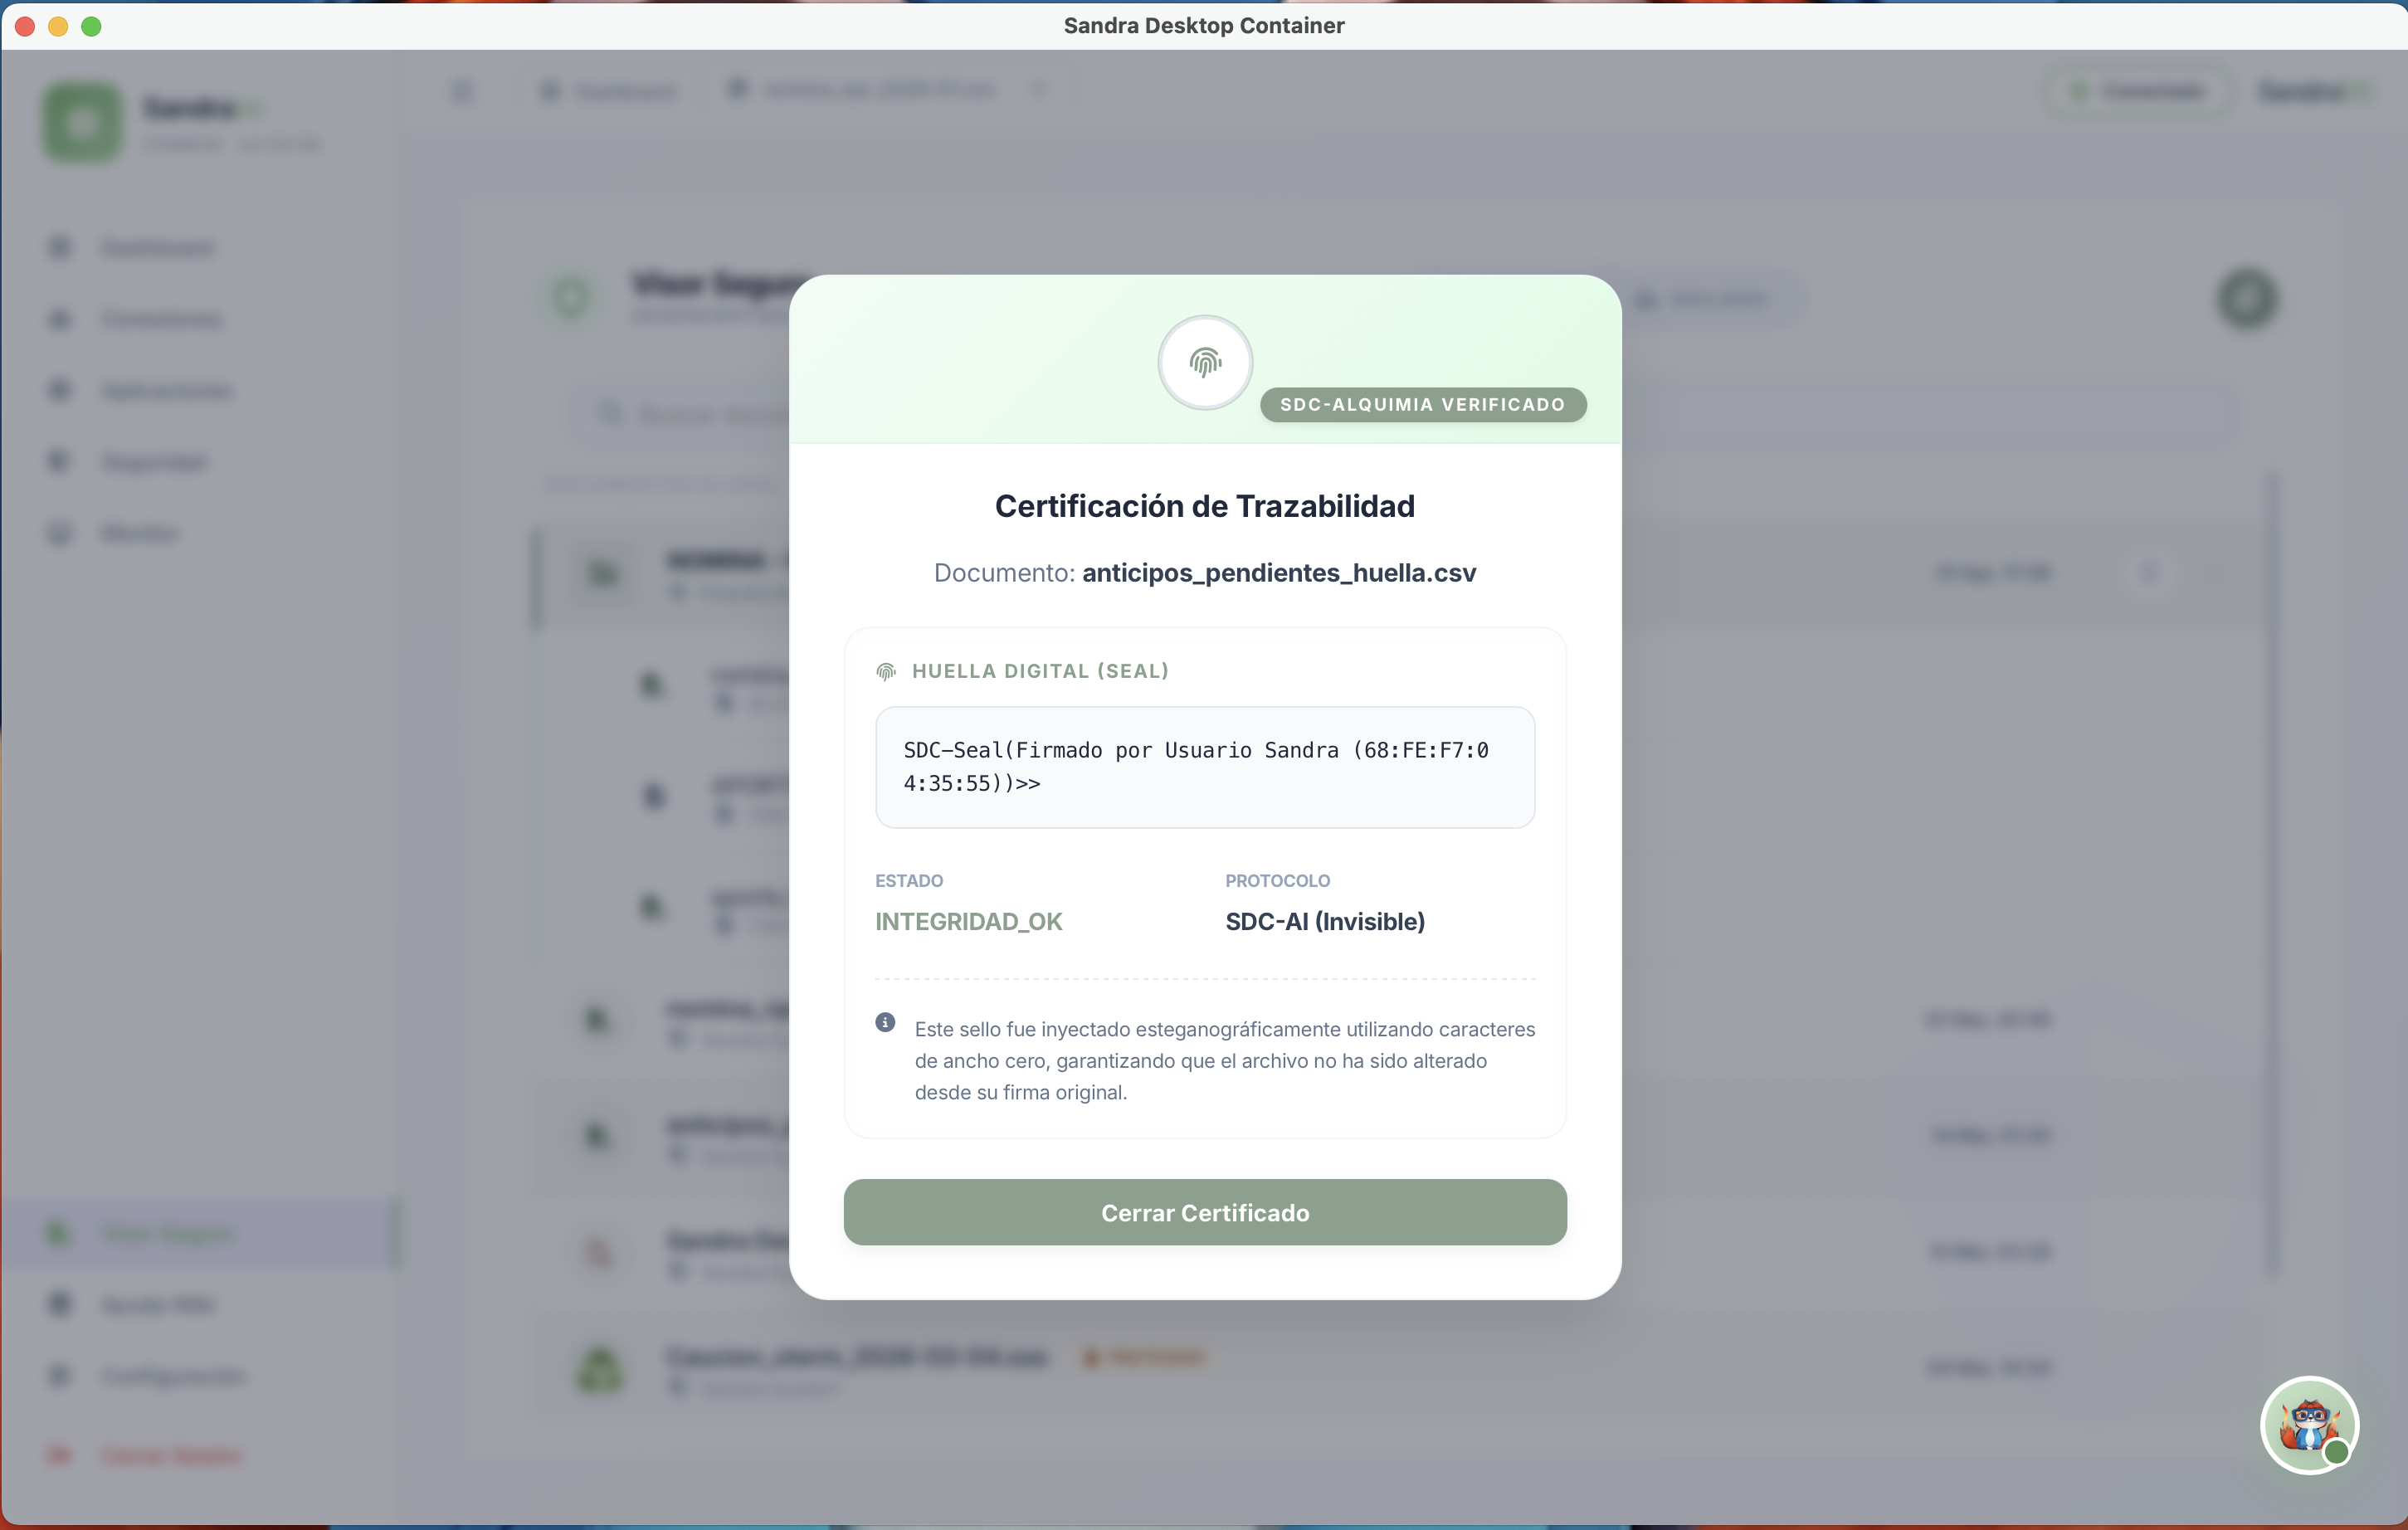
\includegraphics[width=0.95\textwidth]{anexos/11 visor.huelladigital.png}
\caption{Activación del sello de trazabilidad en el Visor de Documentos}
\label{fig:visor-huella}
\end{figure}

\notacientifica{Desde el Visor, el usuario puede activar o desactivar el sellado según sus necesidades. Por defecto, el sistema está configurado para sellar automáticamente todos los documentos exportados.}

\subsection{Huella Digital del Documento}

Cuando se visualiza un documento en SDC, el sistema muestra su "huella digital":

\begin{caja}{Información Mostrada}
\begin{itemize}
\item \textbf{Hash de contenido}: Identificador único del contenido
\item \textbf{Estado del sello}: Activo/Inactivo/Inválido
\item \textbf{Fecha de creación}: Cuando fue generado el documento
\item \textbf{Origen}: Usuario y dispositivo que lo crearon
\item \textbf{Trazabilidad}: Historial de movimientos del documento
\end{itemize}
\end{caja}

Esta información permite al usuario saber instantáneamente si un documento está protegido por Alquimia Invisible.

\section{Conclusiones del Capítulo}
\label{sec:ai-conclusiones}

El protocolo Alquimia Invisible representa una innovación significativa en la protección de información sensible:

\begin{caja}{Resumen de Capacidades}
\begin{enumerate}
\item \textbf{Seguridad Imperceptible}: Los sellos son invisibles al usuario pero verificables por el sistema
\item \textbf{Cumplimiento Normativo}: Implementa controles de ISO 27001, ISO 24760 y COBIT 2019
\item \textbf{Trazabilidad Completa}: Cada archivo puede rastrearse hasta su origen
\item \textbf{No Repudiación}: Evidencia criptográfica de autoría
\item \textbf{Resistencia a Manipulación}: Cualquier modificación invalida el sello
\item \textbf{Interoperabilidad}: Compatible con múltiples formatos y sistemas
\end{enumerate}
\end{caja}

\notacientifica{La combinación de técnicas criptográficas avanzadas con esteganografía moderna crea una capa de protección que complementa los mecanismos tradicionales de seguridad, proporcionando capacidades de auditoría y trazabilidad sin precedentes.}

\bigskip

\begin{caja}{Consideraciones Finales}
\begin{itemize}
\item La Alquimia Invisible no reemplaza el cifrado tradicional, sino que lo complementa
\item El protocolo es especialmente valioso en entornos donde la trazabilidad es más importante que la confidencialidad
\item La implementación requiere un equilibrio entre nivel de detalle del sello y tamaño del archivo
\item La educación del usuario sobre la existencia del sistema puede actuar como elemento disuasorio
\end{itemize}
\end{caja}
